\documentclass[10pt]{beamer}
\usepackage[T2A]{fontenc}
\usepackage[utf8]{inputenc}
\usepackage[english,russian]{babel}

\usepackage{amssymb,amsfonts,amsmath}
\usepackage{cite,enumerate,float,indentfirst}
\usepackage{graphicx}
\usepackage{hyperref}
% Цвета для гиперссылок
\definecolor{linkcolor}{HTML}{799B03} % цвет ссылок
\definecolor{urlcolor}{HTML}{799B03} % цвет гиперссылок

% \hypersetup{pdfstartview=FitH,  linkcolor=linkcolor,urlcolor=urlcolor, colorlinks=true}
\hypersetup{unicode=true}

\graphicspath{{images/}}
\DeclareGraphicsExtensions{.pdf,.png,.jpg}
\usepackage{graphicx}
\usepackage{colortbl}
\usepackage{xcolor}
\usepackage{ifthen}
\usepackage{subfigure}
\usepackage{amsthm}
\usepackage{listings} % code format pasting
\lstset{language=Mathematica}
\lstset{basicstyle={\sffamily\scriptsize},
    numbers=left,
    numberstyle=\tiny\color{gray},
    numbersep=5pt,
    breaklines=true,
    captionpos={t},
    frame={lines},
    rulecolor=\color{black},
    framerule=0.5pt,
    columns=flexible,
    tabsize=2
}

% Some themes
\usetheme{Hannover}
% \usetheme{Madrid}
\usefonttheme{professionalfonts}

\title[]{Семинар: кривые второго порядка}
\author[]{Абдуллин Рустам Фаритович}
\institute[НГУ]
{
    \vspace{0.5cm}
    \begin{minipage}{0.6\linewidth}
        \begin{center}
            \scriptsize
            \textbf{ НОВОСИБИРСКИЙ ГОСУДАРСТВЕННЫЙ УНИВЕРСИТЕТ, НГУ}
        \end{center}
    \end{minipage}
}
\date{\today}

\setbeamertemplate{navigation symbols}{}
\begin{document}
    \begin{frame}
        \titlepage
    \end{frame}

    \section*{Outline}
    \begin{frame}
        \tableofcontents
    \end{frame}

    \section{Повторение}
    \begin{frame}
        \frametitle{Тригонометрическая запись комплексного числа}
        \begin{align*}
            z & = a + b i & r & = \sqrt{a^2 + b^2} \\
            z & = r(\cos \varphi + i \sin \varphi) & \varphi & = \operatorname{arg}(z)
        \end{align*}
        Уравнения для нахождения аргумента:
        \begin{equation*}
            \left\{
                \begin{aligned}
                    \sin \varphi &= \frac{b}{r} = \frac{b}{\sqrt{a^2 + b^2}} \\
                    \cos \varphi &= \frac{a}{r} = \frac{a}{\sqrt{a^2 + b^2}}
                \end{aligned}
            \right.
            \qquad
            \begin{aligned}
                \sin \varphi & = \sin (\pi - \varphi), \\
                \cos \varphi & = \cos (-\varphi), \\
                \tan \varphi & = \tan (\pi + \varphi).
            \end{aligned}
        \end{equation*}
    \end{frame}

    \begin{frame}
        \frametitle{Тангенс угла}
        \begin{figure}
            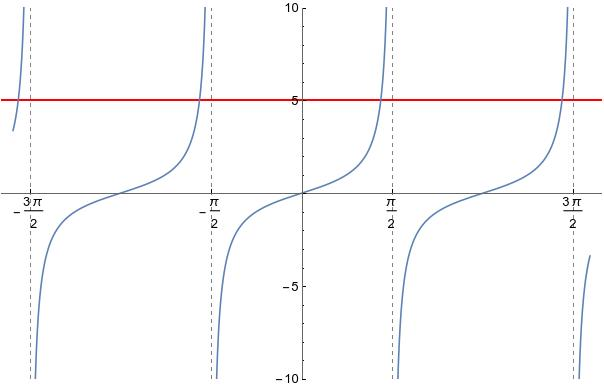
\includegraphics[width=\textwidth]{tangent.jpg}
        \end{figure}
    \end{frame}

    \section{Кривые второго порядка на плоскости}
    \subsection{Общий вид уравнения}
    \begin{frame}
        \frametitle{Общий вид уравнения}
        \textbf{Кривая второго порядка} -- это фигура, точки которой удовлетворяют уравнению
        \begin{equation}
            a_{11}x^2 + 2a_{12}xy+a_{22}y^2 + 2a_{13}x + 2a_{23}y + a_{33} = 0,
        \end{equation}
        где по крайней мере один из коэффициентов $a_{11}$, $a_{12}$, $a_{22}$ не равен нулю.

        Характеристическая квадратичная форма кривой второго порядка 
        \begin{equation}
            F(x,y) = a_{11}x^2 + 2a_{12}xy+a_{22}y^2
        \end{equation}
    \end{frame}

    \begin{frame}[fragile]
        \begin{columns}
            \begin{column}{0.5\textwidth}
                \begin{figure}
                    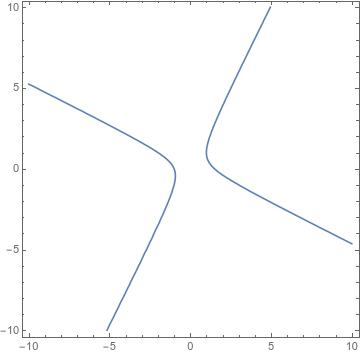
\includegraphics[width=\textwidth]{hyperbola.jpg}
                \end{figure}
            \end{column}

            \begin{column}{0.4\textwidth}
                \begin{equation*}
                    2 x^2+3 x y-x-2 y^2+y-3 = 0
                \end{equation*}
                \href{https://www.wolframalpha.com/}{\textbf{WolframAlpha}}
            \end{column}
        \end{columns}
        \begin{lstlisting}[language=Mathematica]
            ContourPlot[2x^2+3x y-2y^2-x+y-3==0,{x,-10,10},{y,-10,10}]
        \end{lstlisting}
    \end{frame}

    \subsection{Классификация кривых второго порядка}
    \begin{frame}
        \frametitle{Классификация кривых второго порядка}
        \begin{center}
            \begin{tabular}{|l|c|}
                \hline
                Эллипс & $ \frac{x^2}{a^2} + \frac{y^2}{b^2} = 1$ \\
                \hline
                Гипербола & $ \frac{x^2}{a^2} - \frac{y^2}{b^2} = 1$ \\
                \hline
                Парабола & $ y^2 = 2px $ \\
                \hline
                Мнимый эллипс (нет решения) & $ \frac{x^2}{a^2} + \frac{y^2}{b^2} = -1$ \\
                \hline
                Пара пересекающихся прямых & $ \frac{x^2}{a^2} - \frac{y^2}{b^2} = 0$ \\
                \hline
                Пара параллельных прямых & $ x^2 - d^2 = 0$ \\
                \hline
            \end{tabular}
        \end{center}
    \end{frame}

    \begin{frame}[fragile]
        \begin{figure}
            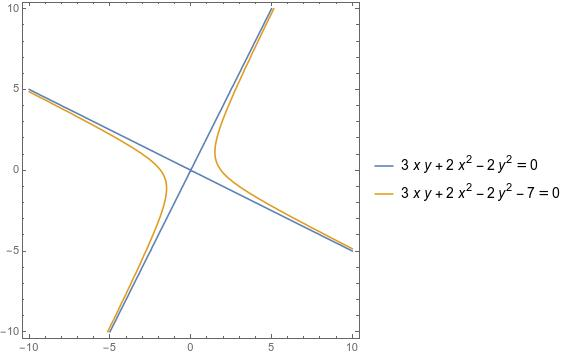
\includegraphics[width=0.7\textwidth]{classification.jpg}
        \end{figure}
        \begin{lstlisting}[language=Mathematica]
            ContourPlot[{2x^2+3x y-2y^2==0,2x^2+3x y-2y^2-7==0},{x,-10,10},{y,-10,10},PlotLegends->"Expressions"]
        \end{lstlisting}
    \end{frame}

    \subsection{Приведение к каноническому виду}
    \begin{frame}
        \frametitle{Определение типа кривой}
        Пусть $a_{11} \neq 0$, тогда получим:
        \begin{equation}
            \begin{aligned}
                F(x,y) & = a_{11}x^2 + 2a_{12}xy+a_{22}y^2 = \\
                & = a_{11}\left(x + \frac{a_{12}}{a_{11}}y \right)^2 + \left(a_{22} - \frac{a_{12}^2}{a_{11}} \right)y^2,
            \end{aligned}
        \end{equation} 
        далее делаем замену координат
        \begin{equation}
            \left\{
                \begin{aligned}
                    x^\prime & = x + \frac{a_{12}}{a_{11}}y \\
                    y^\prime & = y
                \end{aligned}
            \right.
            \qquad
            F(x^\prime, y^\prime) = a_{11}x^{\prime 2} + \left(a_{22} - \frac{a_{12}^2}{a_{11}} \right)y^{\prime 2}
        \end{equation}
    \end{frame}

    \begin{frame}
        \frametitle{Определение типа кривой}
        Обозначим
        \begin{equation}
            a = a_{11}, \qquad b = a_{22} - \frac{a_{12}^2}{a_{11}}
        \end{equation}
        тогда возможны следующие варианты:
        \begin{enumerate}
            \item $a$ и $b$ имеют \textbf{одинаковый} знак ($\operatorname{sgn}(a) = \operatorname{sgn}(b)$), 
            тогда кривая имеет эллиптический тип (\textit{эллипс, мнимый эллипс})
            \item один из коэффициентов равен нулю, тогда кривая имеет параболический тип
            \item $a$ и $b$ имеют \textbf{разный} знак ($\operatorname{sgn}(a) = - \operatorname{sgn}(b)$), тогда кривая имеет гиперболический тип
        \end{enumerate}
    \end{frame}

    \begin{frame}
        \frametitle{Примеры}
        \begin{equation}
            2x^2+3x y-2y^2-x+y-3=0
        \end{equation}
    
        \begin{equation}
            \begin{aligned}
                F(x,y) & = 2x^2 + 3x y-2y^2 = 2\left(x + \frac{3}{4}y \right)^2 - \left(2 + \frac{9}{8}\right)y^2 \\
                & = 2x^{\prime 2} - \frac{25}{8} y^{\prime 2},
            \end{aligned}
        \end{equation} 
        \begin{equation}
            \begin{aligned}
                x^\prime & = x + \frac{3}{4}y \\
                y^\prime & = y
            \end{aligned}
            \qquad
            \qquad
            \begin{aligned}
                x & = x^\prime - \frac{3}{4}y^\prime \\
                y & = y^\prime
            \end{aligned}
        \end{equation}
    \end{frame}
    
    \begin{frame}
        \frametitle{Примеры}
        \begin{equation}
            \begin{aligned}
                & 2x^{\prime 2} - \frac{25}{8} y^{\prime 2} - \left(x^\prime - \frac{3}{4}y^\prime\right) + y^\prime - 3 = \\
                & = 2 \left(x^\prime - \frac{1}{4} \right)^2 - \frac{25}{8}\left(y^\prime - \frac{7}{25}\right)^2-\frac{576}{200} = 0.
            \end{aligned}
        \end{equation}
        отсюда видно, что заданная кривая, это гипербола.
        В случае, если $a_{11} = a_{22} = 0$, то сначала можно сделать замену $y = x + y^\prime$
        \begin{equation*}
            xy = 1
            \qquad
            \begin{aligned}
                x & = x^\prime \\
                y & = x^\prime + y^\prime
            \end{aligned}
            \Longrightarrow 
            x^\prime (x^\prime + y^\prime) = x^{\prime 2} +  x^\prime y^\prime = 1
        \end{equation*}
        \noindent\makebox[\linewidth]{\rule{\textwidth}{0.4pt}}
        \begin{equation*}
            xy = 1
            \qquad
            \begin{aligned}
                x & = x^\prime - y^\prime \\
                y & = x^\prime + y^\prime
            \end{aligned}
            \Longrightarrow 
            (x^\prime - y^\prime)(x^\prime + y^\prime) = x^{\prime 2} - y^{\prime 2} = 1
        \end{equation*}
    \end{frame}

    \subsection{Параметрическое задание кривых второго порядка}
    \begin{frame}
        \frametitle{Параметрическое задание кривых второго порядка}
        \begin{equation*}
            \begin{aligned}
                \frac{x^2}{a^2} + \frac{y^2}{b^2} & =1 \\
                \cos^2 t + \sin^2 t & =1 
            \end{aligned}
            \Longrightarrow
            \left\{
            \begin{aligned}
                x & = a \cos t \\
                y & = b \sin t 
            \end{aligned}
            \right.
        \end{equation*}

        \noindent\makebox[\linewidth]{\rule{\textwidth}{0.4pt}}

        \begin{equation*}
            \begin{aligned}
                \frac{x^2}{a^2} - \frac{y^2}{b^2} & =1 \\
                \operatorname{ch}^2 t - \operatorname{sh}^2 t & =1 
            \end{aligned}
            \Longrightarrow
            \left\{
            \begin{aligned}
                x & = \pm a \operatorname{ch} t & = \pm a\frac{e^x+e^{-x}}{2} \\
                y & = b \operatorname{sh} t & = b\frac{e^x-e^{-x}}{2} 
            \end{aligned}
            \right.
        \end{equation*}

        \noindent\makebox[\linewidth]{\rule{\textwidth}{0.4pt}}

        \begin{equation*}
            y^2 = 2px
            \Longrightarrow
            \left\{
            \begin{aligned}
                x & = \frac{t^2}{2p} \\
                y & = t 
            \end{aligned}
            \right.
        \end{equation*}
    \end{frame}

    \section{Homework}
    \begin{frame}
        \frametitle{Homework}
        \begin{itemize}
            \item \textit{Гюнтер, Кузьмин. Задачник по ВМ.} № 254, 255, 256, 257
            \item Определите тип кривой на комплексной плоскости, которая задается уравнением:
            \begin{enumerate}
                \item $|z-i|=1$
                \item $|z-1|+|z+1|=3$
                \item $|z-i|-|z+i|=1$
            \end{enumerate}
        \end{itemize}
    \end{frame}

\end{document}